\documentclass[12pt]{article}
\usepackage{graphicx}
\usepackage{amsmath}
\usepackage{mathtools}
\usepackage{gensymb}

\newcommand{\mydet}[1]{\ensuremath{\begin{vmatrix}#1\end{vmatrix}}}
\providecommand{\brak}[1]{\ensuremath{\left(#1\right)}}
\providecommand{\norm}[1]{\left\lVert#1\right\rVert}
\newcommand{\solution}{\noindent \textbf{Solution: }}
\newcommand{\myvec}[1]{\ensuremath{\begin{pmatrix}#1\end{pmatrix}}}
\let\vec\mathbf

\begin{document}
\begin{center}
\textbf\large{CHAPTER-11 \\ CIRCLES}

\end{center}
\section{Excercise 11.1}
Find the equation of the circle with centre $(-a,-b)$ and radius $\sqrt{a^2-b^2}$.

\section{SOLUTION}
Given points are
\begin{align}
	\vec{c} = \myvec{-a\\-b} \text{ and } r = \sqrt{a^2-b^2}
\end{align}
The equation of the circle 
\begin{align}
	\norm{\vec{x}}^{2} + 2\vec{u}^{\top}\vec{x} + f = 0
\end{align}
\begin{align}
	\vec{u} &= \myvec{a\\b}\\
	f &= \norm{\vec{u}}^2 - r^2\\
	  &= \myvec{a^2+b^2-a^2-b^2}\\
	  &=2b^2
\end{align}
Thus ,the equation of circle is obtained as
\begin{align}
	\norm{\vec{x}}^2 +2 \myvec{a&b}\vec{x}+2b^2 &= 0       		       
\end{align}	
\section{FIGURE}
Assume the values in (a,b) for plot the figure in python
\begin{align}
\vec{c}=\myvec{3\\2} \text{ and } r=\sqrt{3^2-2^2}
\end{align} 
\begin{figure}[h]
\centering
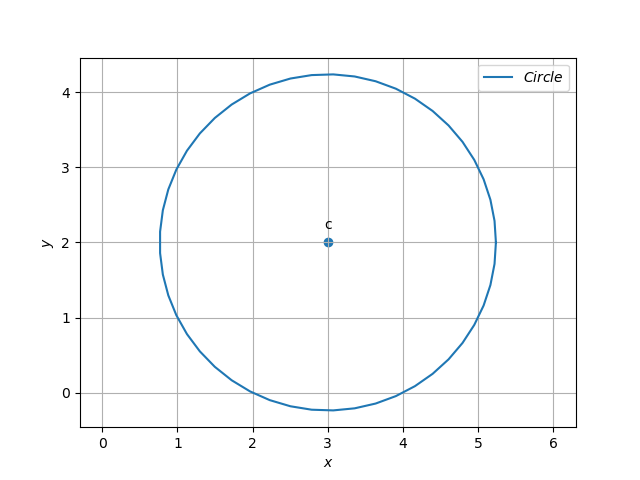
\includegraphics[width=\columnwidth]{circle.png}
\caption{circle}
		\label{fig:Figure}
\end{figure}
   \end{document}